% !TeX document class: article
% !TeX spellcheck: en_US
%
% File: 11M_Functions_Notes_20250819.tex
% Description: Notes on the properties of various types of functions, including polynomial and exponential.
% Keywords: math, functions, algebra, polynomial, exponential
% Date: August 19, 2025
% Author: [Your Name]
\documentclass[tikz, border=5mm]{standalone}

% ----- Encoding and Font Setup (for pdfLaTeX) -----
% T1 font encoding for better hyphenation and broader character support.
\usepackage[T1]{fontenc}
% Input encoding for your source files (UTF-8 is standard for modern editors).
\usepackage[utf8]{inputenc}
% Latin Modern provides a high-quality, vectorized version of Computer Modern.
\usepackage{lmodern}

% ----- Microtype for Enhanced Typography (Optional but Recommended) -----
% Improves spacing and appearance of text and math, even in small elements.
\usepackage[final]{microtype}
\microtypesetup{protrusion=true, expansion=true, tracking=true}
\UseMicrotypeSet[protrusion]{basicmath} % Apply microtype to math as well

% ----- Colors -----
% Robust color package for defining and using colors in your diagrams.
\usepackage{xcolor}

% ----- Mathematics Packages -----
% amsmath: Essential for advanced mathematical typesetting (e.g., align environment).
% fleqn: Ensures equations are left-aligned (consistent with your other documents).
\usepackage[fleqn]{amsmath}
% amsfonts & amssymb: Provide additional math fonts (e.g., Blackboard Bold) and symbols.
\usepackage{amsfonts, amssymb}
% physics: Provides convenient macros for physics (e.g., \qty, \vec, \abs, \dv, \pdv).
\usepackage{physics}
% For declaring custom math operators (e.g., cosec).
\DeclareMathOperator{\cosec}{cosec}

% ----- TikZ and PGFPlots Configuration -----
% tikz: The core package for creating vector graphics.
\usepackage{tikz}
% tkz-euclide: For Euclidean geometry constructions within TikZ.
\usepackage{tkz-euclide}
% pgfplots & pgfplotstable: For creating publication-quality plots from data or functions.
\usepackage{pgfplots, pgfplotstable}
% circuitikz: For drawing electrical circuit diagrams (useful in physics).
\usepackage[americanvoltages,fulldiodes,siunitx]{circuitikz}
% tikz-3dplot: For 3D coordinate systems and drawing in 3D (useful for vectors, solids).
\usepackage{tikz-3dplot}

% tikz: Load common libraries for various drawing tasks.
\usetikzlibrary{
    patterns,          % For filling shapes with patterns
    arrows.meta,       % Modern arrow tip definitions
    calc,              % For coordinate calculations
    arrows,            % Older arrow definitions (can sometimes be useful, meta is preferred)
    shadows.blur,      % For blurred shadows
    math,              % For math parsing within TikZ
    angles,            % For drawing angles
    shapes.geometric   % For predefined geometric shapes
}

% pgfplots: Set compatibility mode for consistent behavior.
\pgfplotsset{compat=1.18}
% pgfplots: Load libraries for statistics and filling areas between plots.
\usepgfplotslibrary{statistics, fillbetween}
% TikZ: Set default arrow style for consistency.
\tikzset{>=latex}

% ----- Image Path -----
% Use the most common path directly, or keep commented options as reminders.
% Uncomment the correct line depending on platform
%\graphicspath{{I:/My Drive/Latex/Images/}} % Windows
%\graphicspath{{D:/Latex/images/}}          % Windows
%\graphicspath{{G:/Other computers/My Computer (1)/latex/images/}} % Laptop
%\graphicspath{{/media/sagar/0E605F52605F401F/latex/images/}} % Linux
\graphicspath{{./Images/}} % Adjust path for your images if different from book's

%=====================================================================
% Document Body: Place your TikZ diagrams here
% Each diagram will typically be within a \begin{tikzpicture} ... \end{tikzpicture}
% The 'standalone' class will automatically crop the PDF to the content.
%=====================================================================
\begin{document}

% Example Diagram: A simple coordinate system with a point and a vector
\begin{tikzpicture}
    % Draw coordinate axes
    \draw[->] (-2,0) -- (2,0) node[right] {$x$};
    \draw[->] (0,-2) -- (0,2) node[above] {$y$};

    % Draw a point P
    \coordinate (P) at (1.5, 1);
    \fill (P) circle (1.5pt) node[above right] {$P(x,y)$};

    % Draw a vector from origin to P
    \draw[->, blue, thick] (0,0) -- (P) node[midway, below left] {$\vec{r}$};

    % Draw a right angle mark
    \tkzMarkRightAngle[fill=gray!20,size=0.2](P,0,1.5,0); % Right angle to x-axis
\end{tikzpicture}

% Another Example: A simple circuit diagram
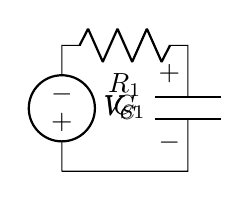
\begin{tikzpicture}[scale=0.8]
    \draw (0,0) to [V, l_=$V_S$] (0,2)
                to [R, l_=$R_1$] (2,2)
                to [C, l_=$C_1$, v_=$V_C$] (2,0)
                to [short] (0,0);
\end{tikzpicture}

% Example of a simple 3D diagram
\tdplotsetmaincoords{70}{110} % Set viewing angles
\begin{tikzpicture}[tdplot_main_coords]
    % Draw axes
    \draw[thick,->] (0,0,0) -- (3,0,0) node[anchor=north east]{$x$};
    \draw[thick,->] (0,0,0) -- (0,3,0) node[anchor=north west]{$y$};
    \draw[thick,->] (0,0,0) -- (0,0,3) node[anchor=south]{$z$};

    % Draw a point P in 3D
    \tdplotsetcoord{P}{2}{30}{60} % Define point P (radius, theta, phi)
    \draw[red,fill=red!50!white] (P) circle (1.5pt);
    \node[red,font=\small] at (P) [above right]{$P$};

    % Project P onto xy plane
    \draw[dashed] (P) -- (P |- 0,0,0) node[below left]{$P_{xy}$};
\end{tikzpicture}


\end{document}